\chapter{Аналитическое изучение устойчивости планарной геликоидальной структуры.}\label{ch:ch3}

Планарная геликоидальная структура описывается парой угловых функций $\theta_0(z) = \pi/2$, $\phi_0(z) = q_0 z$ with $z\in[0,\,L]$.
Для определения устойчивости этой структуры нужно изучить вторую вариацию свободной энергии на этой структуре, $\delta^2\FF_\mathrm{tot}(\theta_0,\phi_0)$. 
Вторая вариация свободной энергии в отсутствие флексоэлектрической поляризации уже была найдена в работе~\cite{VAR2013}:
\begin{multline}\label{eq:F2_on_planar_helicoidal}
\left.\delta^2\FF_{\text{tot}}\right|_{\bar{e}=0}
=\frac{S_{\!\bot}}{2}\bigg[\int_{0}^{L}
\left(K_{11}(\delta\theta')^2+M\delta\theta^2+K_{22}(\delta\phi')^2\right)\, dz +\\
+\sum_{\alpha=1,2}W_\theta^{(\alpha)}\delta\theta^2(l_\alpha)
+\sum_{\alpha=1,2}W_\phi^{(\alpha)}\delta\phi^2(l_\alpha)\bigg],
\end{multline}
где
\begin{equation}
M = K_{33}q_0^2 - \varepsilon_a U^2/(4\pi L^2).
\end{equation}
Так как $J_1\big|_{\theta = \theta_0}=0$ и $\delta J_1\big|_{\theta = \theta_0}=0$, то вклад во вторую вариацию свободной энергии, обусловленный флексоэлектрической поляризацией, даётся выражением
\begin{equation}\label{get_d2Flex}
\delta^2\FF_{\mathrm{flex}}
=-S_{\!\bot}\bar{e} (U/L) \delta\theta^2\Big|_0^L.
\end{equation}
Следовательно, вторая вариация свободной энергии $\delta^2\FF_\mathrm{tot}=\left.\delta^2\FF_{\text{tot}}\right|_{\bar{e}=0} + \delta^2\FF_{\mathrm{flex}}$ оказывается суммой двух независимых вариаций по углам $\theta$ и $\phi$.
При этом часть, зависящая от вариации $\phi$, положительно определена, так как $K_{22}>0$ and $W^{(1,2)}_\varphi>0$.
Таким образом, устойчивость планарной геликоидальной струтктуры определяется только членами, зависящими от вариации $\theta$:

\begin{equation}\label{d2F_theta}
\delta^2 \FF_\theta =
\frac{S_{\!\bot}}{2}\int_{0}^{L}\left(K_{11}(\delta\theta')^2 + M(\delta\theta)^2\right) dz + \frac{S_{\!\bot}}{2}\sum_{\alpha=1,2}
\EuScript{W}^{(\alpha)}
\delta\theta^2(l_\alpha),
\end{equation}
где
\begin{equation}\label{W_renorm}
\EuScript{W}^{(\alpha)}=W_\theta^{(\alpha)} - 2(-1)^\alpha\bar{e} U/L.
\end{equation}
Вклад флексоэлектрической поляризации во вторую вариацию свободной энергии $\delta^2\FF_\text{tot}$ сводится к ренормированию модулей сцепления с поверхностью, $W_\theta^{(\alpha)}\rightarrow \EuScript{W}^{(\alpha)}$.
Следует отметить, что один из эффективных модулей зацепления $\EuScript{W}^{(\alpha)}$ с ростом приложенного напряжения $U$ увеличивается и остаётся положительным, в то время как другой уменьшается и при достаточно больших значениях $U$ становится отрицательным.
Введём следующие обозначения:
\begin{equation}\label{Wtheta_eff_pm}
\EuScript{W}^{+} =
\begin{cases}
\EuScript{W}^{(1)},&\mbox{if } U >0,\\
\EuScript{W}^{(2)},& \mbox{if } U<0,
\end{cases}\quad
\EuScript{W}^{-} =
\begin{cases}
\EuScript{W}^{(2)},& \mbox{if } U >0,\\
\EuScript{W}^{(1)},& \mbox{if } U<0.
\end{cases}
\end{equation}
Как следует из выражения~\eqref{d2F_theta}, планарная геликоидальная структура может стать неустойчивой только если хотя бы один из параметров $\{M, \EuScript{W}^{-}\}$ отрицателен.
В дальнейшем в этой главе ограничимся рассмотрением случая положительной анизотропии диэлектрической проницаемости, $\epsilon_a > 0$.
Таким образом, неустойчивось возможна в следующих ситуациях:
\begin{equation}\label{3_instability_conditions_W}
\begin{aligned}
\centering
\mathrm{I}. &&M < 0,\quad & \EuScript{W}^{-} \geq  0,\\
\mathrm{II}. && M < 0,\quad &\EuScript{W}^{-} < 0,\\
\mathrm{III}. && M \geq 0,\quad &\EuScript{W}^{-} < 0.\\
\end{aligned}
\end{equation}
Условия~\eqref{3_instability_conditions_W} можно записать в виде неравенств для напряжения $U$:
\begin{equation}
\begin{split}
&\mathrm{I}.\quad U_e< \left|U\right| \leq U_\mathrm{flex},\\
&\mathrm{II}.\; \left|U\right|> \max( U_e, U_\mathrm{flex}),\\
&\mathrm{III}.\; U_\mathrm{flex}< \left|U\right| \leq U_e.
\end{split}
\label{eq:conditions_for_voltages}
\end{equation}
Здесь введены обозначения:
\begin{equation}\label{UfrUfl}
U_e =2 q_0 L \sqrt{\frac{\pi K_{33}}{\varepsilon_a}}, \;
U_\mathrm{flex}=
\frac{L}{2\bar{e}}
\begin{cases}
W_\theta^{(2)},&\!\! \text{if } U >0,\\
W_\theta^{(1)},&\!\!\text{if } U<0.
\end{cases}
\end{equation}
Области на плоскости $(\bar{e},\,U)$, соответствующие этим неравенствам, изображены на Рис.~\ref{pic:Zones}.

Представим $\delta \theta(z)$ в виде суммы двух слагаемых:
\begin{equation}\label{thetamupsi}
\delta\theta(z) = \delta\psi(z) + \delta\mu(z),
\end{equation}
где
\begin{equation}\label{mu0=muL=0}
\delta\mu(0) = \delta\mu(L) = 0.
\end{equation}
\todo{Функция $\delta\psi(z)=\delta\psi(z,\delta_1,\delta_2)$ выбрана как решение следующего дифференциального уравнения с граничными условиями:}
\begin{equation}
\begin{cases}
K_{11} \delta\psi''(z) - M\delta\psi(z) = 0,\\
\delta\psi(0) = \delta_1,\ \delta\psi(L) = \delta_2.
\end{cases}
\label{eq:diff_system}
\end{equation}
Такой выбор $\delta\mu(z)$ и $\delta\psi(z)$ даёт возможность разделить интегральный член в~\eqref{d2F_theta}, на два слагаемых, по отдельности зависящих от этих функций; выполнение первого условия в~\eqref{eq:diff_system} позволяет исключить ``перекрёстный член'' после подстановки $\delta\psi(z)$ и $\delta\mu(z)$ в~\eqref{d2F_theta}.

Решение уравнения~\eqref{eq:diff_system} может быть представлено в следующем виде:
\begin{equation}\label{psi=}
\delta\psi =
\begin{cases}
\displaystyle\delta_1\frac{\sin \xi(L-z)}{\sin\xi L}+\delta_2\frac{\sin\xi z}{\sin\xi L},&\quad M < 0,\hspace{-4mm} \\
\displaystyle\delta_1 (L - {z})/{L} + \delta_2{z}/{L},\hspace{-4mm} &\quad M = 0,\\
\displaystyle\delta_1\frac{\sinh \xi(L-z)}{\sinh\xi L}+\delta_2\frac{\sinh\xi z}{\sinh\xi L},\hspace{-4mm} &\quad M > 0,\\
\end{cases}
\end{equation}
где обратная длина $\xi$ определяется как
\begin{equation}\label{xi=}
\xi = \sqrt{\left|M\right|K_{11}^{-1}} = \sqrt{\left|K_{33}q_0^2-\varepsilon_a U^2/(4\pi L^2)\right|K_{11}^{-1}}.
\end{equation}
Разделяя $\delta\theta$ на два слачаемых, даваемых выражениями~\eqref{thetamupsi} и~\eqref{psi=}, представим $\delta^2\FF_\theta$ в виде суммы двух независимых квадратичных форм
\begin{equation}
\delta^2 \FF_\theta =\frac{1}{2}S_{\!\bot}( Q_\psi + Q_\mu),
\label{eq:separation_into_two_modes}
\end{equation}
где
\begin{eqnarray}\label{Qdelta0}
\hspace{-7mm}&&Q_\psi= \int_{0}^{L}\left(K_{11}\delta\psi'^2(z)+M\delta\psi^2(z)\right)\mathrm{d}z
+\!\sum_{\alpha=1,2}\EuScript{W}^{(\alpha)}\delta_\alpha^2,\\
\hspace{-7mm}&&Q_\mu=\int_{0}^{L}\left(K_{11}(\delta\mu')^2+M(\delta\mu)^2\right)\mathrm{d}z.\label{Qmu}
\end{eqnarray}
Стоит отметить, что только $Q_\psi$ зависит от искажений на границе $\delta_{1,2}$.
Идея такого разделения вариации на часть, зависящую от вариации функции в объёме и часть, зависящую от, в том числе, граничных вариаций, впервые была применена Фейнманом~\cite{Feynman}.
Сейчас эта идея широко используется при описании ячеек ЖК~\cite{VRR2001, Kiselev2004, VAR2013}.
Так как $K_{11}>0$, квадратичная форма $Q_\mu$ определена положительно, если $M\geq 0$ ($|U|\leq U_e$).
Однако условие $M \geq 0$ можно ослабить, так как вариации $\delta\mu$ и $\delta\mu'$ связаны.
Для этого представи $\mu(z)$ в виде ряда Фурье на интервале $[0; \, L]$.
Принимая во внимание граничные условия~\eqref{mu0=muL=0}, удобно записать ряд Фурье только по синусам
\begin{equation}\label{sine_expansion}
\mu(z)=\sum\limits_{m=1}^{\infty}c_m \sin{\frac{\pi m z}{L}}\,,
\end{equation}
так как каждое слагаемое в~\eqref{sine_expansion} обращается в ноль при $z=0$ и $z=L$. 
Подставляя разложение~\eqref{sine_expansion} в~\eqref{Qmu}, получаем
\begin{equation}\label{4.1.2.6n}
Q_\mu=\frac{L}{4}\sum\limits_{m=1}^{\infty}
c_m^2\left[K_{11}\left(\frac{\pi m}{L}\right)^2+M\right]\,.
\end{equation}
Условие положительной определённости $Q_\mu$ эквивалентно положительности всех коэффициентов 
\begin{equation}\label{coeffs_at_cm}
K_{11}\left(\frac{\pi m}{L}\right)^2 + M,\ m \geq 1,
\end{equation}
так как $c_m$ могут принимать произвольные значения.
Заметим, что значения коэффициентов~\eqref{coeffs_at_cm} растут с увеличением $m$, так как $K_{11} > 0$.
Таким образом, положительность всех коэффициентов определяется положительностью первого из них:
\begin{equation*}
\left(\frac{\pi}{L}\right)^2K_{11} + M > 0,
\end{equation*}
что, учитывая определение $\xi$~\eqref{xi=}, позволяет записать~\autocite{VAR2013}
\begin{equation}\label{xiL<pi}
\xi L < \pi.
\end{equation}
Подставляя~\eqref{psi=} в~\eqref{Qdelta0}, получаем
\begin{equation}\label{eq:Q_psi_final}
Q_\psi=
\begin{cases}
\begin{aligned}\sum\limits_{\alpha=1,2}\left(K_{11}\xi \cot{\xi L}+\EuScript{W}^{(\alpha)}\right) \delta_\alpha^2 - \\
\phantom{\sum_{a}}
- 2K_{11}(\xi/\sin\xi L)\delta_1\delta_2,
\end{aligned}&\text{при } M<0,\\
\begin{aligned}\sum\limits_{\alpha=1,2}\left(K_{11}/L
+\EuScript{W}^{(\alpha)}\right) \delta_\alpha^2 - \qquad\\
\phantom{\sum_{a}}-  2(K_{11}/L)\delta_1\delta_2,
\end{aligned}&\text{при } M=0,\\
\begin{aligned}
\sum\limits_{\alpha=1,2}\left(K_{11}\xi \coth{\xi L}+\EuScript{W}^{(\alpha)}\right) \delta_\alpha^2 - \\
- 2K_{11} (\xi/\sinh\xi L)\delta_1\delta_2,
\end{aligned}& \text{при } M>0.
\end{cases}
\end{equation}
Используя критерий Сильвестра для $Q_\psi$ и учитывая неравенство~\eqref{xiL<pi}, получаем условия устойчивости планарной геликоидльной структуры ХЖК:
\begin{subequations}\label{eq:ineq_all_M_final}
\begin{align}
&\text{при}\; |U|>U_e:\,
\begin{cases}
{ 0< t} < \pi,\\
w^{+}+t\cot t>0,\\
w^{(1)}w^{(2)}+2\bar{w} t \cot {t}> t^2,
\end{cases}\label{eq:ineq_M<0_final_a}\\
&\text{при}\; |U|=U_e:\,
\begin{cases}
t = 0,\\
w^{+}+1>0,\\
w^{(1)}w^{(2)}+2\bar{w}> 0,
\end{cases}\label{eq:ineq_M=0_final_b}\\
&\text{при}\; |U|<U_e:\,
\begin{cases}
{ t>0,}\\
w^{+}+ t\coth t>0,\\
w^{(1)}w^{(2)}+2\bar{w}  t \coth t>- t^2,
\end{cases}\label{eq:ineq_M>0_final_c}
\end{align}
\end{subequations}
где введены безразмерные параметры $t = \xi L$, $w^{+}={\EuScript{W}^{+} L}/{K_{11}}$, $w^{(\alpha)}={\EuScript{W}^{(\alpha)} L}/{K_{11}}$, и $\bar{w}=({W}^{(1)}_\theta+{W}^{(2)}_\theta)L/2K_{11}$.
Покажем, что каждая из систем неравенств~\eqref{eq:ineq_all_M_final} может быть сведена к одному неравенству.
Рассмотрим систему неравенств~\eqref{eq:ineq_M<0_final_a} и сравним первое и второе.
Для этого построим график функции $f(t) = t \cot{t} + w^{+}$ на интервале $t\in(0,\, \pi)$ (см. Рис.~\ref{pic:graphs_for_inequalities}).
Видно, что решение неравенства $f(t) > 0$ -- интервал $(0, t')$, где $t'$ -- корень уравнения $f(t) = 0$, причём $t'\in(\pi/2,\, \pi)$.
Таким образом, выполнение второго неравенства гарантирует выполнение первого (при этом условие $t>0$ естественным образом следует из определения $t$).
\begin{figure}\label{pic:graphs_for_inequalities}
	\centering
	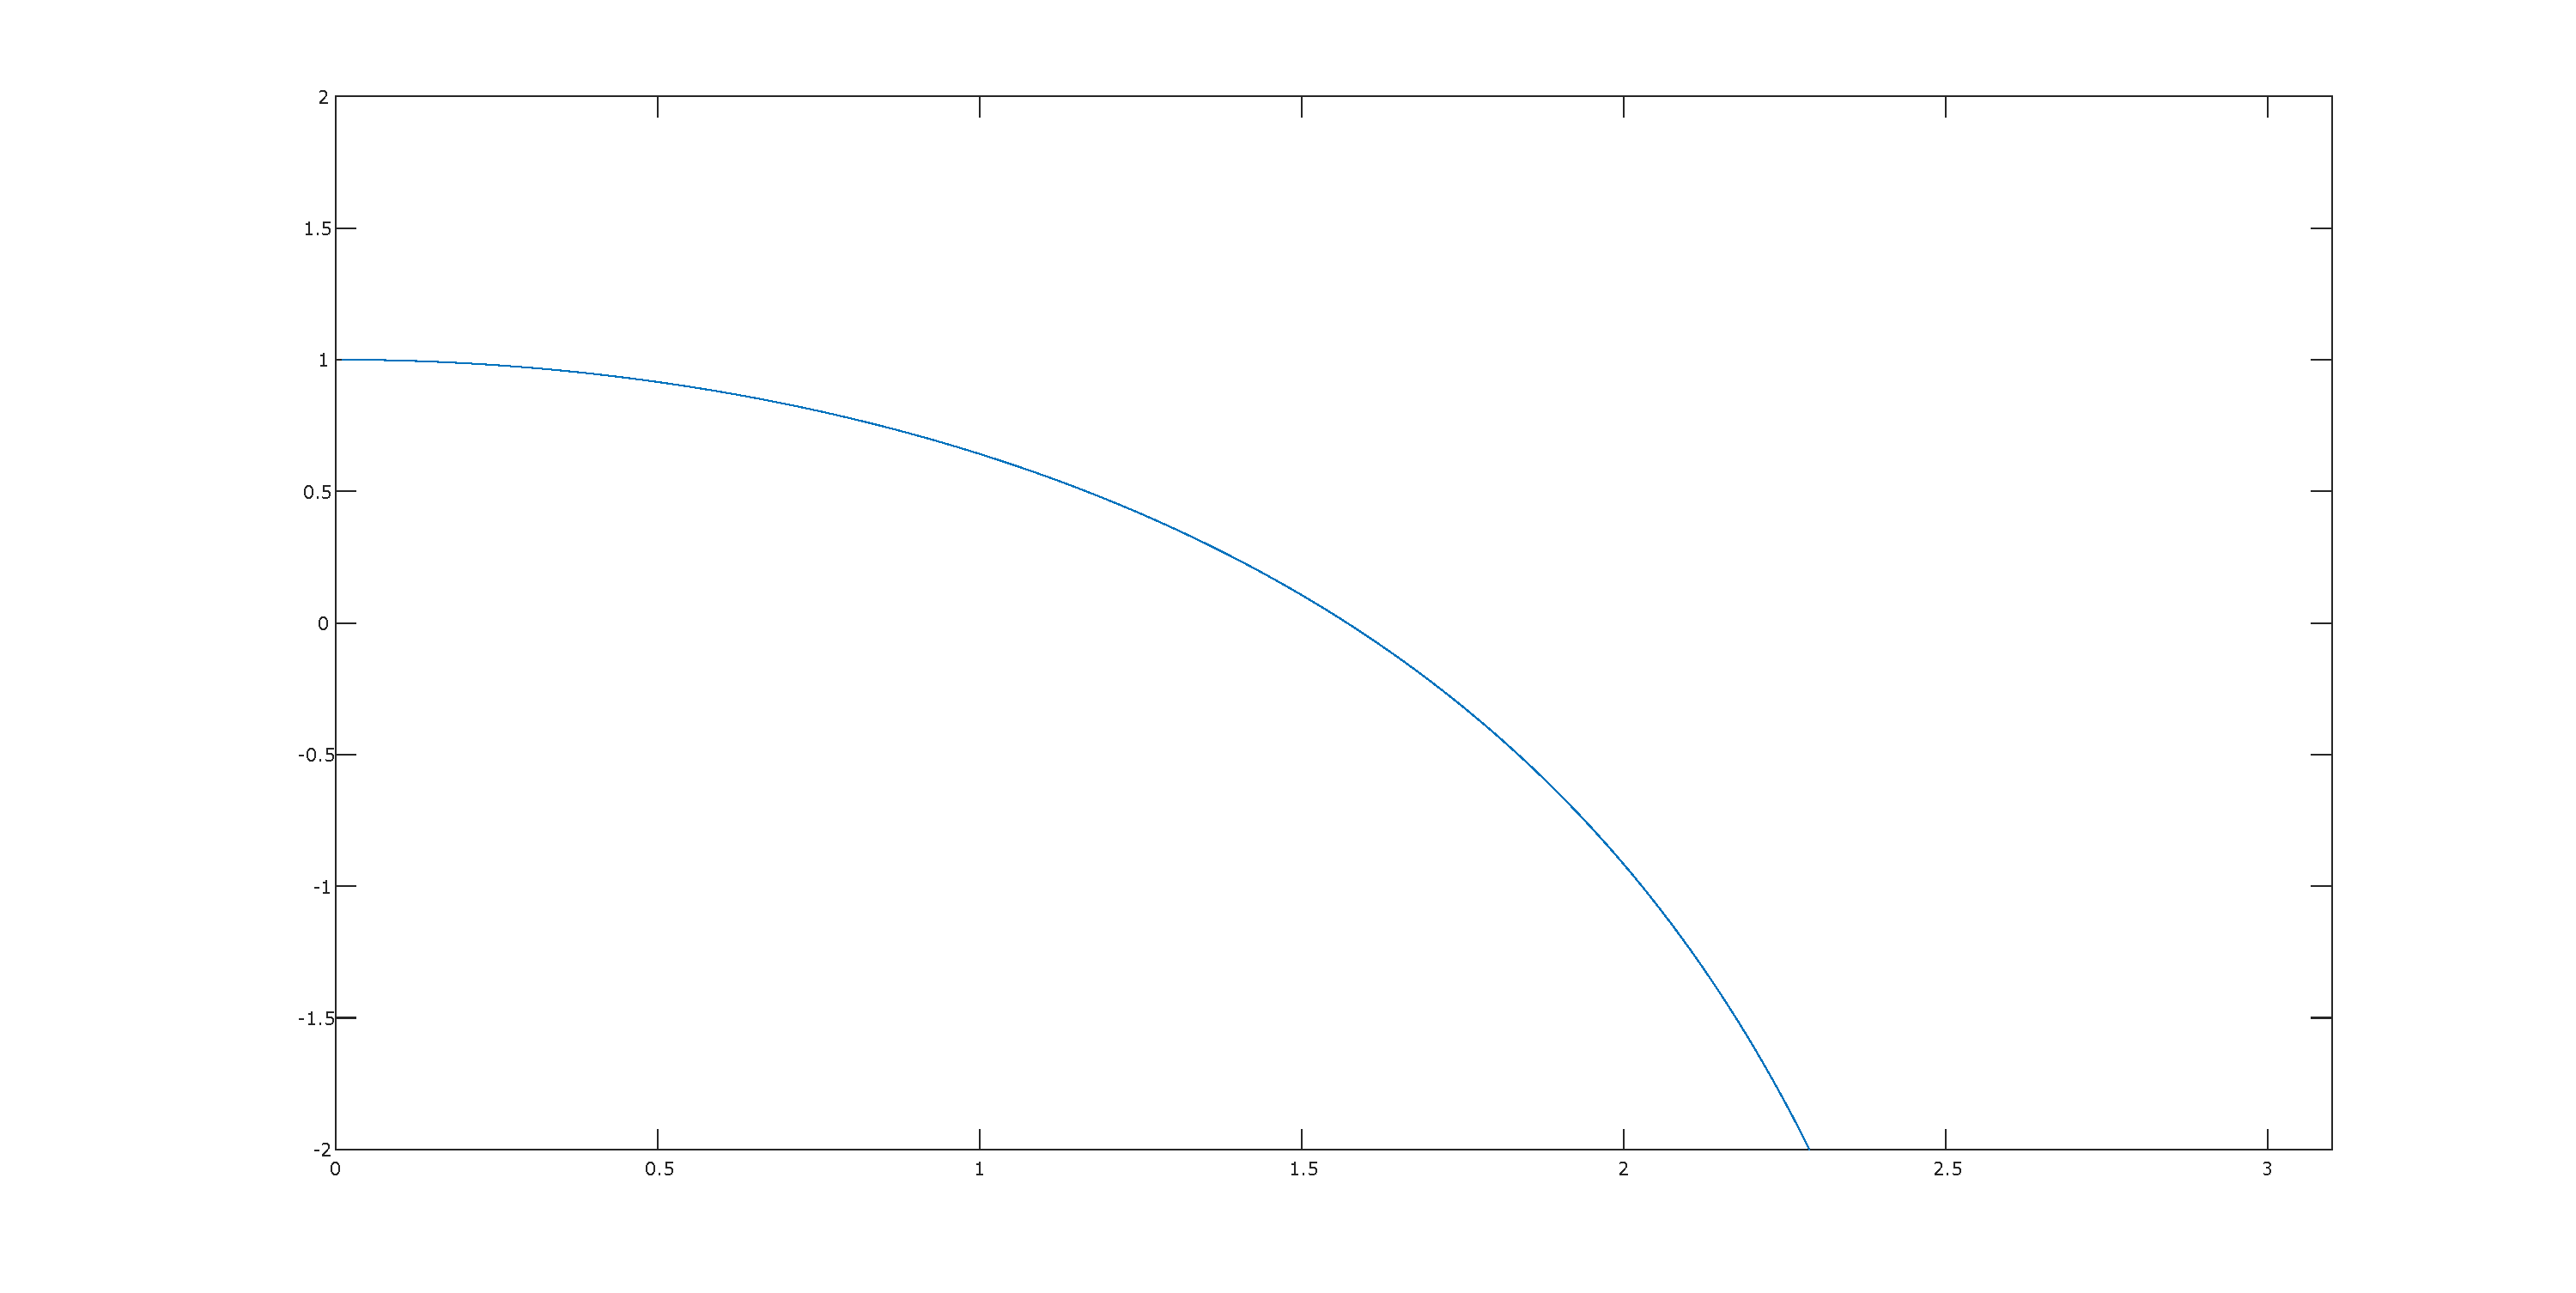
\includegraphics[width = 10cm]{drawing.eps}
	\caption{Some Caption}
\end{figure}
Для сравнения второго неравенства с третьим умножим второе на $2\bar{w}$, получим:
\begin{equation}
w^{+}w^{-} + (w^{+})^2 + 2\bar{w} t\cot{t} > 0.
\end{equation}
Обозначая $F(t) = w^{+}w^{-} + 2\bar{w} t\cot{t}$, можно переписать второе и третье неравенства в следующем виде:
\begin{equation}
\begin{cases}
(w^{+})^2 + F(t) > 0\\
F(t) - t^2 > 0.
\end{cases}
\end{equation}
Видно, что при выполнении последнего неравенства (соответственно, третьего в~\eqref{eq:ineq_M<0_final_a}) второе также выполняется.
Далее, нетрудно видеть, что первое и второе неравенства в системах~\eqref{eq:ineq_M=0_final_b} и~\eqref{eq:ineq_M>0_final_c} выполняются при любых возможных значениях $t$ и $w^{+}$.
Таким образом, мы показали, что последнее неравенство в каждой из систем в~\eqref{eq:ineq_all_M_final} определяющее, а значит, является критерием устойчивости:
\begin{equation}\label{stab_cond_final}
\begin{aligned}
&w^{(1)}w^{(2)}+2\bar{w} t \cot{t}- t^2>0,\hspace{-2mm} & \text{if}\; |U|>U_e,\\
&w^{(1)}w^{(2)}+2\bar{w} > 0, \hspace{-2mm} &\text{if}\; |U|=U_e,\\
&w^{(1)}w^{(2)}+2\bar{w}   t \coth t+ t^2>0, \hspace{-2mm}  &\text{if}\; |U|<U_e.
\end{aligned}
\end{equation}
\begin{subequations}\label{eqU*analitic}
Неравенства~\eqref{stab_cond_final} трансцендентны относительно напряжения $U$, содержащегося в $t=\xi L$, где $\xi$ даётся выражением~\eqref{xi=}. Однако $\bar{e}$ входит только в $w^{(\alpha)} = \EuScript{W}^{(\alpha)}L/K_{11}$, где $\EuScript{W}^{(\alpha)}$ даются выражением~\eqref{W_renorm}.
Таким образом, неравенства~\eqref{stab_cond_final} квадратичны относительно $\bar{e}$, и условия устойчивости могут быть записаны явно:
\begin{align}
&0\leq \bar{e}\leq+\infty,\!\!  &&\text{если }U = 0, \label{eq:interval_1}\\
&0\leq \bar{e} < e_+^*,\!\!  &&\text{если }0<|U|<U_{1},\label{eq:interval_2}\\
&e_-^*< \bar{e} < e_+^*,\!\!  &&\text{если }U_{1} \leq |U|<U_2,\,  U\Delta{w} > 0,\label{eqU*analitic3}\\
&\bar{e}\in\varnothing,\!\!  &&\text{если }U_{1} \leq |U|<U_2, \,  U\Delta{w} < 0, \label{eqU*analitic4}\\
&\bar{e}\in\varnothing,\!\! &&\text{если }|U| \geq U_2,
\end{align}
\end{subequations}
где $ \Delta{w}=({W}^{(2)}_\theta-{W}^{(1)}_\theta)L/K_{11}$,
\begin{equation}\label{eq:!!}
e_\pm^*(U)=\left(K_{11}/4U\right)\left(\Delta{w}
\pm 2\bar{w}\sgn{U}\sqrt{ 1+X(U) }\right) ,
\end{equation}
\begin{equation}\label{eq:!!!}
X(U)=\frac{2}{\bar{w}}\times
\begin{cases}
\displaystyle t\cot t-{t^2}/2\bar{w}, \hspace{-0mm} & \mbox{if } |U|>U_e, \\
\displaystyle 1,\phantom{A^B_C} \hspace{-0mm} & \mbox{if } |U|=U_e, \\
\displaystyle t\coth t +{t^2}/2\bar{w}, \hspace{-0mm}& \mbox{if } |U|<U_e,
\end{cases}
\end{equation}
а
\begin{equation*}
U_i = \sqrt{4\pi K_{11}\varepsilon_a^{-1}t_i^2 + U_e^2}, \quad i=1,2.
\end{equation*}
Здесь $t_1,t_2\in(0;\pi)$ -- корни уравнений
\begin{equation}\label{eq-s1}
2t\cot t-{t^2}/\bar{w}=-{w}_H\quad \text{и}\quad t\tan (t/2)=\bar{w}
\end{equation}
соответственно,	
\begin{equation*}
{w}_H=\frac{2{W}^{(1)}_\theta{W}^{(2)}_\theta}{{W}^{(1)}_\theta+{W}^{(2)}_\theta}\frac{L}{K_{11}}.
\end{equation*}
Первое из уравнений~\eqref{eq-s1} возникает из требования $e_+^* = 0$ или  $e_-^* = 0$, а второе соответствует условию $1+X(U)=0$.
Заметим, что в случае симметричных энергий сцепления с границей напряжения $U_1$ и $U_2$ одинаковы, и условия~\eqref{eqU*analitic3} и~\eqref{eqU*analitic4} исчезают.

Асимптотики $t_1$ можно записать в следующем виде:
\begin{equation}
t_1\sim
\begin{cases}
\vspace{0.1cm}
\pi\left(1+\frac{2}{{w}_H}-\pi^2\left(\frac{8}{3{w}_H^3}-\frac{2}{\bar{w}{w}_H^2}\right)
\right)^{-1},\! &\!\! {w}_H\gg 1,\\
\vspace{0.1cm}
\frac{\pi}{2}+\frac{{w}_H}{\pi} -\frac{\pi}{4\bar{w}}-\frac{2{w}_H^2}{\pi^3}+\frac{\pi}{8\bar{w}^2}
,\! &\!\! {w}_H\ll 1\ll\bar{w},\\
\left(\frac{1}{2\bar{w}}+\frac13-\frac{{w}_H}{4\bar{w}}+\frac{2\bar{w}}{45}
-\frac{{w}_H}{6}+\frac{{w}_H^2}{8\bar{w}}
\right)^{-1/2},\! &\!\!  \bar{w}\ll 1.
\end{cases}
\end{equation}
Для корня $t_2$ существует предложенная в работе~\autocite{VAR2013} аппроксимация
\begin{equation}
t_2\cong
\begin{cases}
\vspace{0.1cm}
\pi\left(1+2\bar{w}^{-1}-2.5\bar{w}^{-3}\right)^{-1}, & \bar{w}\geq 3.3, \\
\left(0.5\bar{w}^{-1}+0.088 \right)^{-1/2}, &\bar{w} < 3.3,
\end{cases}
\end{equation}
причём точность этой формулы превышает 0.5\% для любых значений $\bar{w}$.

На Рис.~\ref{pic:Zones} на плоскости $(\bar{e}, U)$ показана построенная по формулам~\eqref{eqU*analitic} область устойчивости планарной геликоидальной структуры; остальные материальные параметры стандартные.
\begin{figure}[htb]
\centering
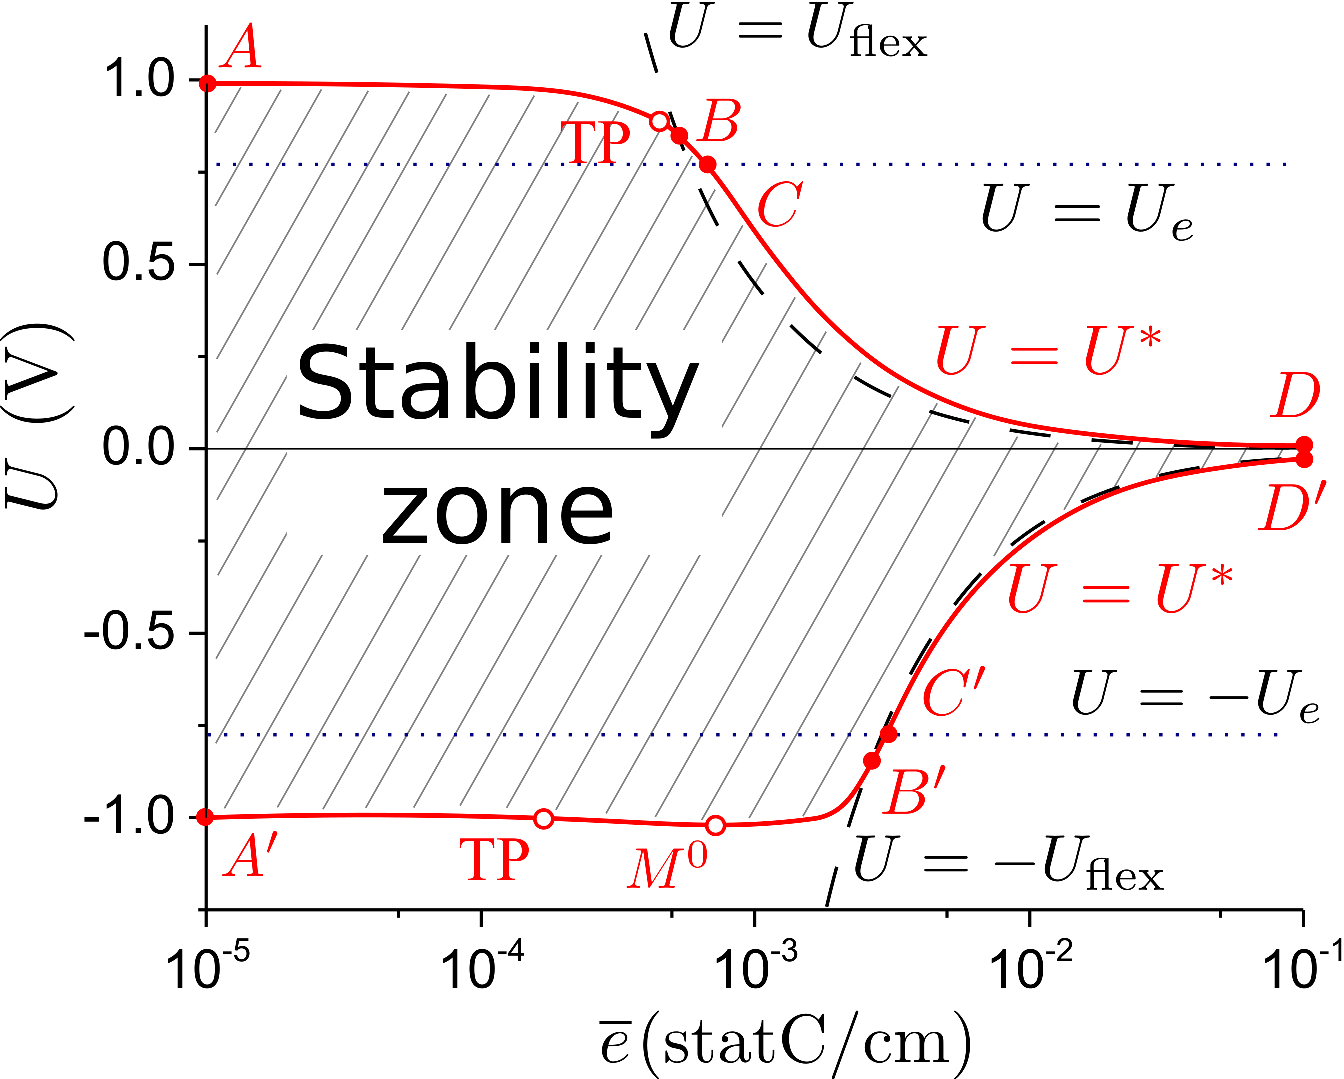
\includegraphics[width = 12cm]{Zones_and_reality_2_plots.eps}
\caption{Кривые $ABCD$ и $A'B'C'D'$, построенные при помощи формул~\eqref{eqU*analitic}, ограничивают область устойчивости планарной геликоидальной ориентационной структуры.}
\label{pic:Zones}
\end{figure}
Область устойчивости расположена между кривыми $ABCD$ и $A'B'C'D'$; они соответствуют напряжению $U = U^*(\bar{e})$.
Зоны неустойчивости планарной геликоидальной структуры расположены выше кривой $ABCD$ и ниже кривой $A'B'C'D'$.
Отметим, что зависимость $U^*$ (см. Рис.~\ref{pic-U_from_e_pos}), полученная при помощи численной минимизации функционала свободной энергии хорошо согласуется с кривой $U^*$, рассчитанной аналитически (см. Рис.~\ref{pic:Zones}).
Участки $AC$ и $A'C'$ соответствуют ситуации, когда первое из неравенств~\eqref{stab_cond_final} становится равенством, а на участках $CD$ и $C'D'$ в равенство обращается третье неравенство из~\eqref{stab_cond_final}.
Физический смысл различных участков кривых $ABCD$ и $A'B'C'D'$ можно объяснить следующим образом.
На участках $AB$ и $A'B'$ энергетически предпочтительны объёмные искажения, а искажения на границе невыгодны.
Напротив, на участках $CD$ и $C'D'$ ориентационные искажения на одной из границ выгодны, а на другой границе и в объёме -- нет.
Наконец, на участках $BC$ и $B'C'$ энергетически предпочтительны искажения в объёме и на одной из границ.
На кривых $ABCD$ и $A'B'C'D'$ знаком ``$\circ$'' отмечены трикритические точки $TP$, а также точка минимума $M^0$.
Существование точки экстремума на одной из кривых $ABCD$ или $A'B'C'D'$ -- это общее свойство систем с несимметричными энергиями сцепления $W_\theta^{(1)}\neq W_\theta^{(2)}$ (минимум на $A'B'C'D'$ при $W_\theta^{(1)}>W_\theta^{(2)}$ и максимум на $ABCD$ при $W_\theta^{(1)}<W_\theta^{(2)}$).
Координаты экстремума $M^0\big(\bar{e}^\circ,U^\circ\big)$ даются выражением
\begin{equation*}
\bar{e}^\circ=\big|{W}^{(2)}_\theta-{W}^{(1)}_\theta\big|L/4U_2,\; U^\circ =U_2\sgn\left(W_\theta^{(2)}-W_\theta^{(1)}\right).
\end{equation*}
Асмиптотика $U^*(\bar{e})$ при $\bar{e}\to\infty$ может быть записана в виде
\begin{equation}\label{A1}
U^*(\bar{e})\sim\left({K_{11}}/{4\bar{e}}\right)\left(\Delta w + 2\bar{w}\sgn(U)\sqrt{ 1+X(0)}\right),
\end{equation}
где
$X(0)=2 (t_0/\bar{w})\coth t_0 +(t_0/\bar{w})^2$, $t_0=q_0L(K_{33}/K_{11})^{1/2}.$
Из выражения~\eqref{A1} для случая $X(0)\ll1$ получаем $U^*\simeq U_\text{flex} \sgn(U)$, следовательно, линии $U^*(\bar{e})$ сближаются с пунктирными линиями на Рис.~\ref{pic:Zones}.
Таким образом, при достаточно больших значениях $\bar{e}$ флексоэлектричество облегчает переход Фредерикса, снижая пороговое напряжение.

\section{Анализ рода перехода Фредерикса при помощи разложения по низшей гармонике в двухпараметрической модели Ландау.}\label{sec:ch3/sec1}

Как показано в предыдущем разделе, планарная геликоидальная ориентационная структура при достижении напряжения $U = U^*$ теряет устойчивость из-за возможности аномального роста флуктуаций ориентации у границ ячейки, описываемых параметрами $\delta_{1,2}$.
Это даёт возможность изучить переход Фредерикса при помощи упрощённой модели, содержащей только моды с $\delta_{1,2}$.
Для этого представим зависимость $\theta(z)$ в виде
\begin{equation}\label{theta_easy}
\tilde\theta(z;\delta_1,\delta_2) = \pi/2 + \delta\psi(z;\delta_1,\delta_2),
\end{equation}
где функция $\delta\psi$ задана выражением~\eqref{psi=}.
Подставляя $\tilde\theta$ в выражение~\eqref{eq:F_for_minimization} и считая $\delta_{1,2} \ll 1$, получаем разложение свободной энергии $\FF_\mathrm{tot}$. Ограничиваясь членами четвёртого порядка малости, запишем
\begin{equation}\label{Landau_general}
\FF_\mathrm{tot}(\delta_1,\delta_2) \approx
\FF^{(0)} + \FF^{(2)}+ \FF^{(4)}=
\FF^{(0)}
+ \frac12\sum\limits_{k=0}^2A_k\delta_1^k\delta_2^{2-k}
+ \frac{1}{4!}\sum\limits_{k=0}^4 B_k\delta_1^k\delta_2^{4-k},
\end{equation}
где $\FF^{(0)}=\FF^{(0)}_f$.
Явные выражения для коэффициентов $A_k$ можно получить из выражения~\eqref{eq:Q_psi_final}:
\begin{align}
&\text{при } M > 0:\quad
	\begin{cases}\label{eq:A_k,M>0}
	A_0 = K_{11}\xi \cot{\xi L}+\EuScript{W}^{(2)}, \\
	A_1 = - 2K_{11}(\xi/\sin\xi L), \\
	A_2 = K_{11}\xi \cot{\xi L}+\EuScript{W}^{(1)},
	\end{cases} \\
&\text{при } M = 0:\quad
	\begin{cases}
	A_0 = K_{11}/L +\EuScript{W}^{(2)},\\
	A_1 = - 2(K_{11}/L),\\
	A_2 = K_{11}/L +\EuScript{W}^{(1)}.
	\end{cases}%\\
%&\text{при } M < 0:\quad
%	\begin{cases}
%	A_0 = K_{11}\xi \coth{\xi L}+\EuScript{W}^{(2)}, \\
%	A_1 = - 2K_{11}(\xi/\sinh\xi L), \\
%	A_2 = K_{11}\xi \coth{\xi L}+\EuScript{W}^{(1)}.
%	\end{cases}
\end{align}
Для случая $M < 0$ формулы для коэффициентов $A_k$ получаются из~\eqref{eq:A_k,M>0} заменой $\sin$ на $\sinh$ и $\cot$ на $\coth$.
Коэффициенты
\begin{equation}
B_k=\partial^4 \FF_\mathrm{tot}(\delta_1,\delta_2)\big/{\partial^k\delta_1 \partial^{4-k}\delta_2}\Big|_{\delta_1=\delta_2=0},
\label{eq:Bk}
\end{equation}
$k=0,\dots ,4$ \todo{Приводятся ниже/в Приложении 1/не приводятся вообще из-за громоздкости?}

Будем считать все параметры системы, кроме напряжения $U$ и усреднённого флексоэлектрического коэффициента $\bar{e}$, зафиксированными.
При достаточно низком напряжении дискриминант $A_1^2-4A_0A_2<0$, и квадратичная форма $\FF^{(2)}$ определена положительно, следовательно, планарная геликоидальная конфигурация устойчива.
С ростом напряжения при фиксированном $\bar{e}$ дискриминант $\FF^{(2)}$ обращается в ноль при $U=U^*(\bar{e})$, и соответствующее неравенство из~\eqref{stab_cond_final} становится равенством.
Наконец, при положительном дискриминанте исследуемая структура неустойчива.
%На Рис.~\ref{pic-U_from_e_pos} и Рис.~\ref{pic:Zones} приведены кривые $U=U^*(\bar{e}),на которых
Cлагаемое $\FF^{(2)}(U, \bar{e})$ обращается в ноль на кривой $U = U^*(\bar{e})$ при $\delta_2=\varkappa_* \delta_1$,
\begin{equation}
\varkappa_*(\bar{e}) = -{A_1(U^*, \bar{e} )}\big/{2A_0(U^*, \bar{e})}.
\end{equation}
Флуктуации директора в планарной геликоидальной ориентации при $U=U^*$ становятся аномально большими.
При этом род перехода (разрывный или непрерывный) определяется знаком слагаемого четвёртого порядка $\FF^{(4)}$ на прямой на плоскости параметров $(\delta_1, \delta_2)$, $\delta_2 = \varkappa_*\delta_1$.
Подставляя $U = U^*$ и $\delta_2 = \varkappa_* \delta_1$ в~\eqref{Landau_general}, получаем
\begin{equation}\label{F_4_sign}
\FF_\mathrm{tot}(\delta_1,\varkappa_*\delta_1) \approx \FF^{(0)} +\frac{1}{4!}\delta_1^4\sum\limits_{k=0}^4 B_k\varkappa_*^k\equiv\FF^{(0)} +\frac{1}{4!}\tilde{B}\delta_1^4.
\end{equation}
При $\tilde{B}=\tilde{B}(\bar{e})> 0$ переход происходит непрерывно.
Напротив, $\tilde{B} < 0$ означает, что система при $U = U^*$ уже находится в искажённом состоянии с энергией, меньшей, чем $\FF^{(0)}$. Следовательно, переход в этом случае разрывный и происходит при $U = U_c$, причём $|U_c| < |U^*|$.
Заметим, что при $\tilde{B}<0$ в модели Ландау требуется учитывать члены разложения шестого или даже более высоких порядков для того, чтобы свободная энергия была положительной при достаточно больших значениях $\delta_{1,2}$~\cite{LLStat1}.
Однако членов четвёртого порядка достаточно для анализа рода перехода.
Отметим, что схожая однопараметрическая модель Ландау для аналогичной ячейки ЖК исследовалась в работе~\cite{VAR2013} для случая $\bar{e} = 0$ с симметричными модулями сцепления с подложкой, $W_\theta^{(1)}=W_\theta^{(2)}$, и в такой системе также обнаруживается как разрывный, так и непрерывный переход.

Координаты трикритической точки $\mathrm{TP}=\left(\bar{e}^\mathrm{TP}, U^\mathrm{TP}\right)$ могут быть найдены из условий
\begin{equation}
U=U^*(\bar{e} ),\; \tilde{B}(\bar{e} )=0,
\end{equation}
причём $\tilde{B}<0$ для $\bar{e}<\bar{e}^\mathrm{TP}$ и $\tilde{B}>0$ при $\bar{e}>\bar{e}^\mathrm{TP}$.
Знак выражения $\tilde{B}(\bar{e})$ можно определить, совмещая~\eqref{theta_easy} и~\eqref{eq:F_for_minimization} и подставляя в~\eqref{eq:Bk}.
Результаты приведены на Рис.~\ref{pic:Landau}.
%Отметим, что при расчёте $\tilde{B}(\bar{e})$ используется напряжение $U^*(\bar{e})$, таким образом, в каждой точке этих зависимостей одинаковы все параметры, кроме напряжения на обкладках -- оно для каждого значения $\bar{e}$ находится отдельно.
Отметим, что на каждой кривой напряжение $U = U^*$ при соответствующем значении $\bar{e}$.
Трикритические точки определяются сменой знака $\tilde{B}$: $\bar{e}^\mathrm{TP}=5.132\times10^{-4}$~Фр/см при $U>0$ и $\bar{e}^\mathrm{TP}=1.676\times10^{-4}$~Фр/см при $U<0$.
Эти точки отмечены на Рис.~\ref{pic:Zones}, и этот результат хорошо согласуется с полученным при помощи численной минимизации свободной энергии (см. Рис.~\ref{pic-U_from_e_pos}).
\begin{figure}
	\centering
	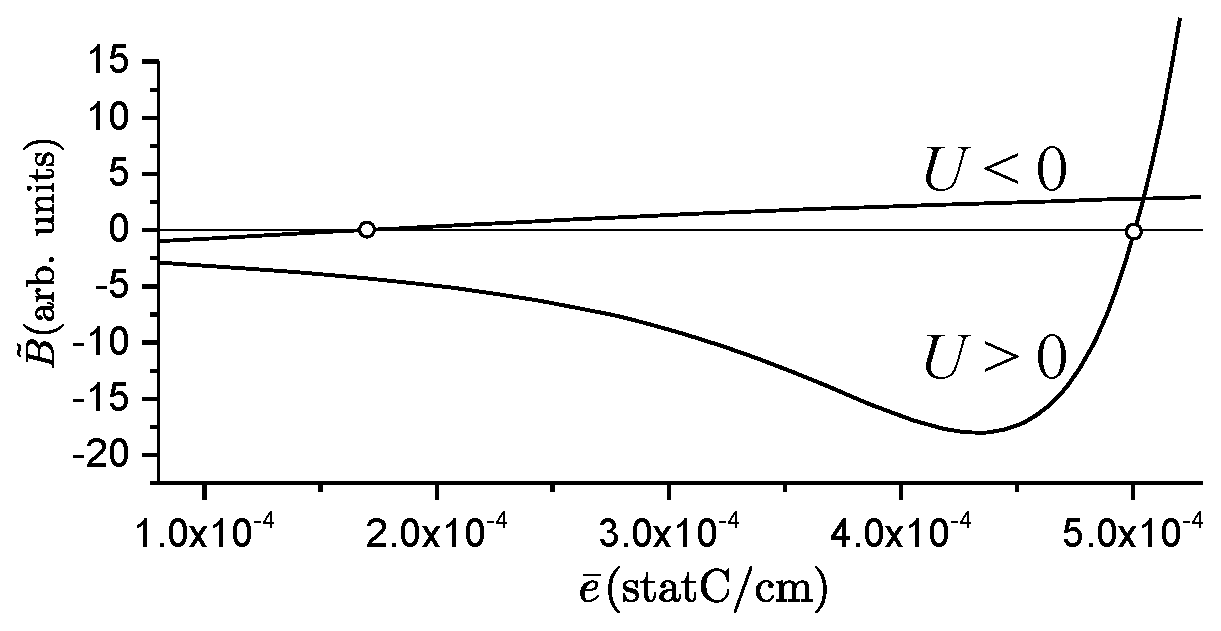
\includegraphics[angle=0,width = 10cm]{B4_pos_and_neg_voltage1.eps}
	\caption{График зависимости эффективного коэффициента $\tilde{B}$ от усреднённого флексоэлектрического коэффициента $\bar{e}$.
		Материальные параметры стандартные.
		Отметки ``$\circ$'' соответствуют трикритическим точкам.
	}
	\label{pic:Landau}
\end{figure}